\documentclass[paper=letter,11pt]{scrartcl}

\KOMAoptions{headinclude=true, footinclude=false}
\KOMAoptions{DIV=14, BCOR=5mm}
\KOMAoptions{numbers=noendperiod}
\KOMAoptions{parskip=half}
\addtokomafont{disposition}{\rmfamily}
\addtokomafont{part}{\LARGE}
\addtokomafont{descriptionlabel}{\rmfamily}
%\setkomafont{pageheadfoot}{\normalsize\sffamily}
\setkomafont{pagehead}{\normalsize\rmfamily}
%\setkomafont{publishers}{\normalsize\rmfamily}
\setkomafont{caption}{\normalfont\small}
\setcapindent{0pt}
\deffootnote[1em]{1em}{1em}{\textsuperscript{\thefootnotemark}\ }


\usepackage{amsmath}
\usepackage[varg]{txfonts}
\usepackage[T1]{fontenc}
\usepackage{graphicx}
\usepackage{xcolor}
\usepackage[american]{babel}
% hyperref is needed in many places, so include it here
\usepackage{hyperref}

\usepackage{xspace}
\usepackage{multirow}
\usepackage{float}


\usepackage{braket}
\usepackage{bbm}
\usepackage{relsize}
\usepackage{tcolorbox}

\def\ketY{\ensuremath{\ket {\Psi}}}
\def\iGeV{\ensuremath{\textrm{GeV}^{-1}}}
%\def\mp{\ensuremath{m_{\textrm{proton}}}}
\def\rp{\ensuremath{r_{\textrm{proton}}}}
\def\me{\ensuremath{m_{\textrm{electron}}}}
\def\aG{\ensuremath{\alpha_G}}
\def\rAtom{\ensuremath{r_{\textrm{atom}}}}
\def\rNucl{\ensuremath{r_{\textrm{nucleus}}}}
\def\GN{\ensuremath{\textrm{G}_\textrm{N}}}
\def\ketX{\ensuremath{\ket{\vec{x}}}}
\def\ve{\ensuremath{\vec{\epsilon}}}


\def\ABCDMatrix{\ensuremath{\begin{pmatrix} A &  B  \\ C  & D \end{pmatrix}}}
\def\xyprime{\ensuremath{\begin{pmatrix} x' \\ y' \end{pmatrix}}}
\def\xyprimeT{\ensuremath{\begin{pmatrix} x' &  y' \end{pmatrix}}}
\def\xy{\ensuremath{\begin{pmatrix} x \\ y \end{pmatrix}}}
\def\xyT{\ensuremath{\begin{pmatrix} x & y \end{pmatrix}}}

\def\IMatrix{\ensuremath{\begin{pmatrix} 0 &  1  \\ -1  & 0 \end{pmatrix}}}
\def\IBoostMatrix{\ensuremath{\begin{pmatrix} 0 &  1  \\ 1  & 0 \end{pmatrix}}}
\def\JThree{\ensuremath{\begin{pmatrix}    0 & -i & 0  \\ i & 0  & 0 \\ 0 & 0 & 0 \end{pmatrix}}} 
\def\JTwo{\ensuremath{\begin{bmatrix}    0 & 0 & -i  \\ 0 & 0  & 0 \\ i & 0 & 0 \end{bmatrix}}}
\def\JOne{\ensuremath{\begin{bmatrix}    0 & 0 & 0  \\ 0 & 0  & -i \\ 0 & i & 0 \end{bmatrix}}}
\def\etamn{\ensuremath{\eta_{\mu\nu}}}
\def\Lmn{\ensuremath{\Lambda^\mu_\nu}}
\def\dmn{\ensuremath{\delta^\mu_\nu}}
\def\wmn{\ensuremath{\omega^\mu_\nu}}
\def\be{\begin{equation*}}
\def\ee{\end{equation*}}
\def\bea{\begin{eqnarray*}}
\def\eea{\end{eqnarray*}}
\def\bi{\begin{itemize}}
\def\ei{\end{itemize}}
\def\fmn{\ensuremath{F_{\mu\nu}}}
\def\fMN{\ensuremath{F^{\mu\nu}}}
\def\bc{\begin{center}}
\def\ec{\end{center}}
\def\nus{$\nu$s}

\def\adagger{\ensuremath{a_{p\sigma}^\dagger}}
\def\lineacross{\noindent\rule{\textwidth}{1pt}}

\newcommand{\multiline}[1] {
\begin{tabular} {|l}
#1
\end{tabular}
}

\newcommand{\multilineNoLine}[1] {
\begin{tabular} {l}
#1
\end{tabular}
}



\newcommand{\lineTwo}[2] {
\begin{tabular} {|l}
#1 \\
#2
\end{tabular}
}

\newcommand{\rmt}[1] {
\textrm{#1}
}


%
% Units
%
\def\m{\ensuremath{\rmt{m}}}
\def\GeV{\ensuremath{\rmt{GeV}}}
\def\pt{\ensuremath{p_\rmt{T}}}


\def\parity{\ensuremath{\mathcal{P}}}

\usepackage{cancel}
\usepackage{ mathrsfs }
\def\bigL{\ensuremath{\mathscr{L}}}

\usepackage{ dsfont }



\usepackage{fancyhdr}
\fancyhf{}


\lhead{\Large 33-444} % \hfill Introduction to Particle Physics \hfill Spring 2019}
\chead{\Large Introduction to Particle Physics} % \hfill Spring 2019}
\rhead{\Large Spring 2022} % \hfill Introduction to Particle Physics \hfill Spring 2019}
\begin{document}
\thispagestyle{fancy}





%\begin{tabular}{c}
%{\large 33-444 \hfill Intro To Particle \hfill Spring 2019\\}
%\hline 
%\end{tabular}

\begin{center}
{\huge \textbf{MidTerm \#2: More Fun Facts}}
\large

\end{center}

{\large

Speed of Light: c = 1  \hspace{1in} Planks constant: $\frac{h}{2\pi} = 1$

$\alpha = 10^{-2}$  \hspace{1in} $\alpha_W$ $\equiv 0.5 \alpha$ \hspace{1in} $\alpha_G$ $\equiv$ $G_N m_p^2$ = $10^{-39}$

GeV$^{-1}$=$10^{-15}$m  \hspace{1in} GeV = $10^{-27}$kg \hspace{1in}   GeV$^{-1} = 6 \cdot 10^{-25}$ s

$r_\textrm{nucleus} \sim 10^{-15}$ meters.

The mass of the electron is $\sim 10^{-3}$ GeV

The mass of the muon is $\sim 10^{-1}$ GeV

The mass of the tauon is $\sim 1$ GeV

The mass of the charm quark is $\sim 1$ GeV

The mass of the bottom quark is $\sim 5$ GeV

The mass of the top quark is $\sim 175$ GeV

The mass of the W-boson $\sim$ mass Z-boson $\sim$ h-boson $\sim 100$ GeV

1 TeV = 1000 GeV

Cross section: $\sigma \sim |M|^2 $  \hspace{1in} Decay rate: $\Gamma \sim |M|^2 $

Life-time: $\tau = \frac{1}{\Gamma}$  

Branching Ratios:  Br(X$\rightarrow$YY) $= \frac{\Gamma(X\rightarrow YY}{\sum_f \Gamma(X\rightarrow ff)}$

\be
\mathscr{L}_{scalar} = \frac{1}{2} (\partial_\mu \phi)(\partial^\mu \phi) + \frac{m^2}{2} \phi^2
\ee

\be
\mathscr{L}_{spin 1/2} = \bar{\psi}(i\gamma_\mu \partial^\mu - m )\psi
\ee

\be
\mathscr{L}_{spin 1} = F_{\mu\nu} F^{\mu\nu}\ \textrm{ where } F_{\mu\nu} = \partial_\mu A_\nu - \partial_\mu A_\nu
\ee

%sagitta:  $\frac{\Delta p_T}{p_T} = \frac{\Delta s}{s}$  \hspace{1in} $\Delta s \sim $ constant $ (\sim 10 \mu m)$ 
%
%Uniform Circular Motion: $r_c = \frac{p_T}{qB}$ 
%
%\begin{figure}[h!]
%\centering
%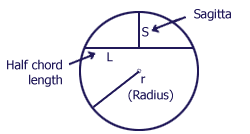
\includegraphics[width=0.3\textwidth]{./Sagitta.png}
%\end{figure}

}





\end{document}
